\chapter{ Packrat Parsing με Ελαστικό Κυλιόμενο Παράθυρο}
\label{ch:elastic}

Όπως αναφέραμε, οι αναλυτές packrat, παρά την απλότητα και την γραμμική επίδοση (ως προς το μήκος της εισόδου) που προσφέρουν, έχουν το μειονέκτημα ότι καταναλώνουν πολύ χώρο για την αποθήκευση των ενδιάμεσων αποτελεσμάτων.
Αυτό αποτελεί αποθαρρυντικό παράγοντα για τη χρησιμοποίησή τους σε πολλές εφαρμογές.
Στην ενότητα αυτή περιγράφουμε μία ευριστική τεχνική για τη βελτίωση της κατανάλωσης μνήμης του packrat parser, χρησιμοποιώντας ένα \textit{κυλιόμενο παράθυρο (packrat parsing with elastic sliding window)} \cite{Kuramitsu2015a}.

\section{Εισαγωγή}

Η ιδέα πίσω από το packrat parsing με ελαστικό κυλιόμενο παράθυρο (ή πιο απλά elastic packrat parsing) βασίζεται στην έννοια του μήκους της μέγιστης οπισθαναχώρησης (longest backtrack length).
Ουσιαστικά, όταν προχωράει ο αναλυτής δεξιότερα ως προς την είσοδο, μπορεί να χρειαστεί να οπισθαναχωρήσει, όχι όμως αναγκαστικά μέχρι την αρχή της εισόδου, αλλά μέχρι ένα μικρότερο μήκος.
Έστω, ότι είχαμε έναν μικρότερο πίνακα υπομνηματισμού (παράθυρο) το οποίο "κυλάει" προς τα δεξιά ως προς την είσοδο και έχει επαρκές πλάτος ώστε να καλύπτει το μήκος της μέγιστης οπισθαναχώρησης. 
Τότε, ο πίνακας αυτός έχει τον απαραίτητο χώρο ώστε να αποθηκεύει όλα τα ενδιάμεσα αποτελέσματα, χωρίς να χρειαστεί οπισθαναχώρηση του αλγορίθμου.

Στην πράξη, βέβαια, είναι δύσκολο να ξέρουμε εκ των προτέρων πόση θα είναι η μέγιστη οπισθαναχώρηση.
Εναλλακτικά, επιλέγουμε ένα προσεγγιστικό μέγεθος για το παράθυρο από εμπειρικά δεδομένα και, αν χρειαστεί, το επεκτείνουμε κατά τη διάρκεια της συντακτικής ανάλυσης.

Όμως, η μέθοδος αυτή δεν περιορίζει μόνο τη χρήση κελιών ως προς τη διάσταση της εισόδου, αλλά και ως προς τη διάσταση των μη τερματικών συμβόλων.
Συγκεκριμένα, κατά την εκτέλεση της συντακτικής ανάλυσης μετριέται δυναμικά κατά πόσο κάθε μη τερματικό αξίζει να αποθηκεύεται στον πίνακα (παράθυρο) ή όχι.
Έτσι, ο χώρος που θα περισσέψει μπορεί να δοθεί ώστε να επεκταθεί το πλάτος του παραθύρου.
Εξ ού, και η "ελαστικότητα" του παραθύρου.

\section{Κυλιόμενο παράθυρο}

To παράθυρο πρακτικά είναι ένας buffer σταθερού μεγέθους, ο οποίος κυλάει προς τα δεξιά ως προς την είσοδο ώστε να περιλάβει τα νέα δεδομένα, ενώ τα παλιά δεδομένα απορρίπτονται από αυτόν. 
To Σχήμα \ref{fig:slide_window} απεικονίζει έναν buffer πλάτους 5 θέσεων πάνω από έναν πίνακα υπομνηματισμού.
Η δεξιότερη θέση του παραθύρου ταυτίζεται με το μέτωπο της συντακτικής ανάλυσης.

\begin{figure}[h]
	\centering
	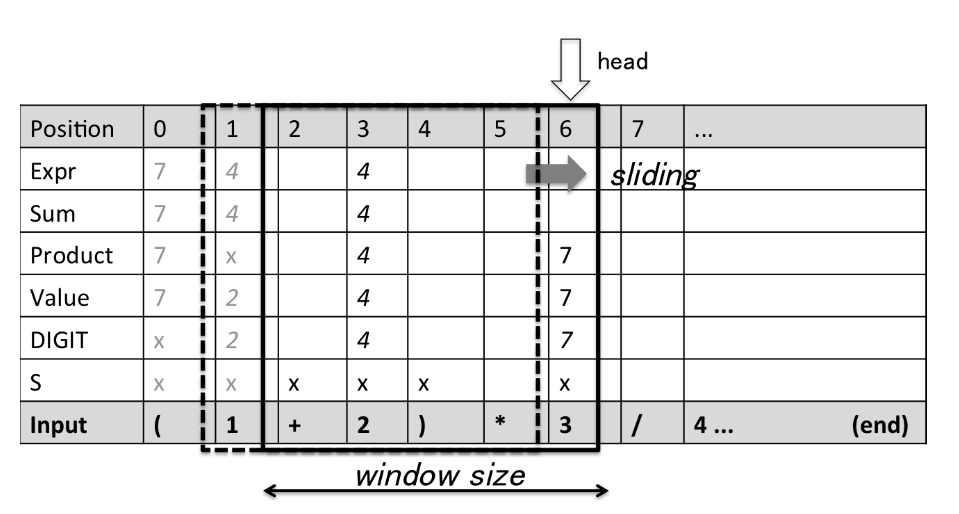
\includegraphics[width=0.8\textwidth]{pics/slide_window} % TODO: how to cite figure from paper
	\caption{Κυλιόμενο παράθυρο για τον πίνακα υπομνηματισμού}
	\label{fig:slide_window}
\end{figure}

Αν το μέγεθος του παραθύρου δεν είναι επαρκώς μεγάλο, τότε θα "εκτοπιστεί" κάποιο χρήσιμο κελί του πίνακα υπομνηματισμού το οποίο περιέχει ένα ενδιάμεσο αποτέλεσμα που στο μέλλον θα χρειαστεί.
Αυτό σημαίνει ότι πρακτικά χάνεται η εγγύηση για γραμμικό χρόνο συντακτικής ανάλυσης, αφού το συγκεκριμένο κελί που χάθηκε θα πρέπει να υπολογιστεί ξανά, όπως θα έκανε ένας αναδρομικός αναλυτής με οπισθαναχώρηση.

Πόσο, όμως, πρέπει να έιναι το πλάτος του παραθύρου, ώστε να αποφευχθεί αυτή η δυσχέρεια?
Αυτή είναι μία δύσκολη ερώτηση. 
Θα μπορούσαμε να το κάνουμε όσο μεγάλο είναι και η είσοδος ώστε να μην ανησυχούμε για το αν θα χάσουμε κάποιο ενδιάμεσο αποτέλεσμα, όμως αυτό είναι ισοδύναμο με την αρχική έκδοση του packrat parsing.
Το άλλο άκρο θα ήταν το πλάτος να είναι $1$, που θα ισοδυναμούσε με έναν αναλυτή αναδρομικής κατάβασης με οπισθαναχώρηση.

Στο \cite{Kuramitsu2015a} παρουσιάζονται πειραματικές μετρήσεις για μία ποικιλία προγραμμάτων σε διάφορες γλώσσες, όπου φαίνεται πως οι πιο πολλές περιπτώσεις οπισθαναχώρησης συμβαίνουν σχετικά κοντά στο μέτωπο της συντακτικής ανάλυσης.
Συγκεκριμένα, ακόμα και ένα παράθυρο μήκους 16 bytes καταφέρνει να αποφύγει τον περιττό υπολογισμό κελιών στο 99.9\% των περιπτώσεων οπισθαναχώρησης.

Το ξεκάθαρο πλεονέκτημα ενός παραθύρου είναι ότι διασφαλίζει ένα άνω φράγμα στη μνήμη που δεσμεύουμε στο σωρό.
Αν μάλιστα το μήκος του παραθύρου είναι επαρκές, τότε εξακολουθεί να ισχύει και η εγγύηση του γραμμικού χρόνου εκτέλεσης.
Ωστόσο, αν όχι, τότε υπάρχει ο κίνδυνος για ακόμα και εκθετικό χρόνο εκτέλεσης ως προς το μήκος της εισόδου, όπως θα έκανε ο αναλυτής αναδρομικής κατάβασης με οπισθαναχώρηση.

\section{Δυναμική απενεργοποίηση μη τερματικών συμβόλων}

Όπως αναφέραμε, στο elastic packrat parsing γίνεται προσπάθεια να περιοριστούν τα ενδιάμεσα αποτελέσματα που αποθηκεύονται, περιορίζοντας όχι μόνο το μήκος της εισόδου που καλύπτουμε, αλλά και τα μη τερματικά που εξυπηρετούμε.
Θα μπορούσαμε να την κάνουμε αυτή την ανάλυση στατικά, όμως η προσέγγιση που επιλέγεται είναι η δυναμική ανάλυση.

Συγκεκριμένα, ξεκινάμε θεωρώντας ότι όλα τα μητερματικά είναι ενεργά, δηλαδή ότι αποθηκεύουμε ενδιάμεσα αποτελέσμα που τα αφορούν.
Στη συνέχεια, αν μετά από έναν συγκεκριμένο αριθμό κλήσεων για ένα μη τερματικό δούμε ότι τα ενδιάμεσα αποτελέσματα που το αφορούν δε χρησιμοποιήθηκαν ούτε μία φορά, το "απενεργοποιούμε".
Δηλαδή, παύουμε να κρατάμε αποτελέσματα για αυτό.

Το ποιο θα είναι αυτό το "κατώφλι", δηλαδή ο αριθμός κλήσεων στο μη τερματικό που δεν αξιοποιεί ούτε ένα ενδιάμεσο αποτέλεσμα, είναι μια παράμετρος που πρέπει να μετρήσουμε.

\section{Elastic Packrat Parsing}

Το elastic packrat parsing είναι μία μέθοδος που συνδυάζει τόσο το κυλιόμενο παράθυρο, όσο και τη δυναμική απενεργοποίηση μη τερματικών.

To Σχήμα \ref{fig:elastic_slide_window} απεικονίζει την ιδέα.

\begin{figure}[h]
	\centering
	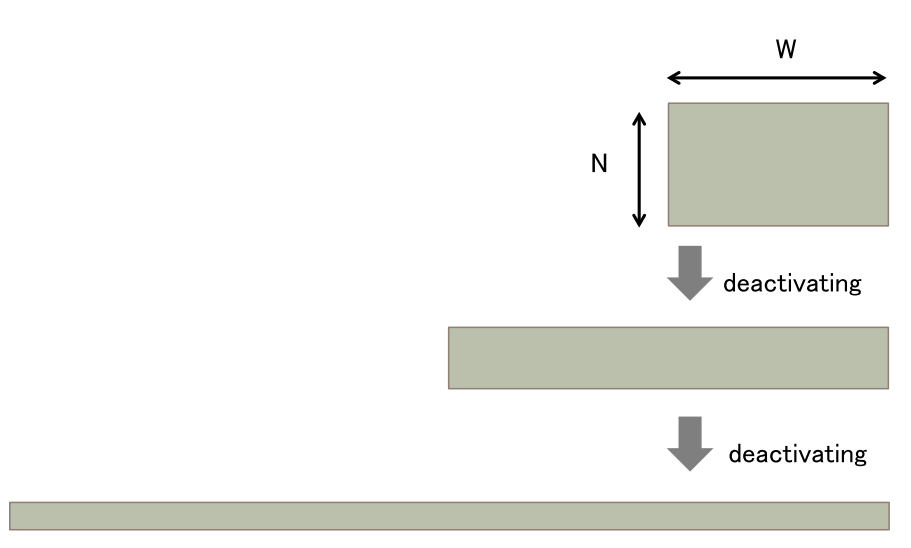
\includegraphics[width=0.8\textwidth]{pics/elastic_slide_window} 
	\caption{Ελαστικό κυλιόμενο παράθυρο}
	\label{fig:elastic_slide_window}
\end{figure}

Για την υλοποίηση, χρησιμοποιούμε έναν μονοδιάστατο πίνακα $W*N$, όπου $W$ είναι το πλάτος του παραθύρου και $N$ ο αριθμός των ενεργών μη τερματικών.
Οπότε, ένα ζεύγος $(position, non terminal)$ αντιστοιχεί σε μία θέση στον μονοδιάστατο πίνακα.
Ακολούθως, χρησιμοποιούμε έναν δείκτη κατακερματισμού (hasing-based index) για να εντοπίσουμε σε ποιο σημείο του μονοδιάστατου πίνακα θα αποθηκευτεί το ενδιάμεσο αποτέλεσμα, όπως στο Σχήμα \ref{fig:elastic_1}.
Φτιάχνουμε, αρχικά, ένα κλειδί μέσω της θέσης και του μη τερματικού, το οποίο μετά το ελαττώνουμε μέσω του modulo ($W*N$).

\begin{figure}[h]
\setlength\partopsep{-\topsep}% adjusts vertical space after the listing
\begin{minted}[frame=lines,linenos,numbersep=5pt]{c++}
    long int key = (pos << shift) | row;
    unsigned int index = hash(key) % (w * n);
    ...
    ElasticCell* cur_cell = &elastic_cells[index];    // πάρε το αντίστοιχο κελί
    cur_cell->set_key(key);        // θέσε το κλειδί στο αντίστοιχο κελί
\end{minted}
\caption{Δημιουργία κλειδιού και δείκτη}
\label{fig:elastic_1}
\end{figure}

Το πλεονέκτημα είναι ότι όταν απενεργοποιούμε ένα μη τερματικό, ο χώρος του στον πίνακα μπορεί να αξιοποιηθεί από άλλα μη τερματικά, διευρύνοντας ουσιαστικά το παράθυρο, όπως δείχνει το Σχήμα \ref{fig:elastic_slide_window}. 
Αυτή είναι και η ουσία της ελαστικότητας της μεθόδου. 
Στην ακραία περίπτωση που μόνο ένα μη τερματικό μείενει ενεργοποιημενο, τότε το παράθυρο έχει πρακτικά μέγεθος ίσο με $W*N$ και τη μορφή μίας γραμμής.

Το μειονέκτημα του hashing-based index είναι πως μπορεί να υπάρχουν συγκρούσεις (collisions) μεταξύ διαφορετικών κλειδιών, που όμως αντιστοιχίζονται στο ίδιο index.
Αυτό αίρει την αυστηρότητα στην αποθήκευση ενδιάμεσων αποτελεσμάτων, αλλά τα οφέλη μίας τέτοιας απλής πρακτικής είναι μεγαλύτερα στη συνήθη περίπτωση.

Τέλος, η τεχνική αυτή δεν περιλαμβάνει ρητή κύλιση του παραθύρου, για πιο απλή υλοποίηση.
Αντίθετα, η κύλιση προς τα δεξιά επιτυγχάνεται έμμεσα, καθώς τα νέα κλειδιά που αποθηκεύονται και αντιστοιχούν σε δεξιότεραρ σημεία της εισοδου, αντικαθιστούν τα παλιά.
Αυτό προσεγγίζει την κύλιση, η οποία θα κόστιζε πολύ περισσότερο σε υλοποιήση για να γίνεται επ'ακριβώς.

